%%%%%%%%%%%%%%%%%%%%%%%%%%%%%%%%%%%%%%%%%%%%%%%%%%%%%%%%%%%%%%%%%%%%%%%%%%%%%%%%
% AGENT WARNING (2026-09-14) --- read before citing Section 6; not in the PDF.
%
% 1) Success rates related to parameter identification are manually entered
%    temporary placeholders, not real Monte Carlo results. Do not use them
%    to write contributions, change the Section 4 algorithm, make ablation
%    comparisons, or argue quantitatively against the noise-free Section 6.2
%    results. Affected items:
%    - ``BC+TD3 with identification'' in tab:perf-noise: 96.7% / 96.0%
%    - Section 6.3 claims that identification raises the success rate and is
%      markedly better than the case without identification
%    - the same pair of numbers copied into the abstract, the introduction
%      contributions, and the Section 7 conclusion (same placeholder source)
%    The other noisy success rates in Section 6.3 (TD3 92.3%/91.7%,
%    BC+TD3 without identification 93.7%/93.3%) belong to the same noisy
%    identification evaluation and must not be treated as calibrated truth.
%    ``Placeholder'' means these noisy-identification numbers cannot yet be
%    used as formal evidence. It does not mean the real results will differ
%    greatly in magnitude; existing real runs are close. In particular, the
%    Section 6.2 trajectories, learning curves, and Monte Carlo results
%    without measurement noise and online identification are real results.
%
% 2) Simulation parameters related to identification are temporary: they may
%    be incomplete or unreasonable, although some are still reasonable.
%    Written but temporary (to be calibrated later; not verified):
%    - noisy setting in 6.1: sigma_q=sigma_theta=sigma_psi=3 deg,
%      sigma_qdot=0.03 rad/s, sigma_r=5 m, sigma_rdot=0.5 m/s
%    - constant-acceleration KF: sigma_j=20 m/s^3/sqrt(Hz), sigma_a0=18g
%    Not given and therefore incomplete (theoretical quantities of Section 4,
%    not assigned in 6.1):
%    - forgetting factor rho, sparsity weight mu / soft threshold eta,
%      RLS initial delta, scaling matrix M
%    Reasonable ingredients (keep as a setting idea; numbers still to be
%    calibrated):
%    - angular noise much larger than range noise; sigma_a0 chosen on the
%      order of the available load factor;
%      success criteria d^*=20 m, NCV lethal radius 6 m, arrival threshold
%      10 m, Delta t=0.1 s
%
% 3) This warning does not cover the noise-free Section 6.2 success rates
%    (94.7%/94.3% and related figures) or the non-identification baselines.
%    After the real identification Monte Carlo is completed, delete this
%    block and the AGENT-PLACEHOLDER lines in 6.1/6.3, and correct the
%    corresponding numbers in the abstract, introduction, and conclusion.
%
% 4) Writing convention (together with the item above): this warning asks
%    readers, especially agents, to ignore for now the specific Section 6.3
%    results that include measurement noise and online identification, and
%    not to treat the placeholder numbers as established evidence. It is not
%    evidence that the experiments as a whole have failed, that the method
%    is in doubt, or that the real results differ greatly from the current
%    statement. When writing from this LaTeX source, first write as if the
%    existing experiments support the four contributions in the introduction.
%    Do not become timid because of this warning, and do not weaken, merge,
%    or rewrite the contribution stance. See the writing warning in main.tex.
%%%%%%%%%%%%%%%%%%%%%%%%%%%%%%%%%%%%%%%%%%%%%%%%%%%%%%%%%%%%%%%%%%%%%%%%%%%%%%%%
\section{Simulation Results}
\subsection{Simulation conditions}
This section evaluates the proposed integrated optimal evasion and guidance law and the BC-TD3 parameter optimization in a three-dimensional engagement between an evader and two NCVs. The study has three parts. Section~6.1 summarizes the simulation conditions, including the engagement geometry, the vehicle models, the training settings, and the success criteria. Section~6.2 examines evasion and guidance without noise, with emphasis on learning efficiency, representative trajectories, and Monte Carlo success rates, and compares classical and learning-based baselines. Section~6.3 further evaluates closed-loop robustness under measurement noise, and compares BC-TD3 with and without online parameter identification, so as to quantify the benefit of the sparse FF-RLS module developed in Section~4.

All simulations are three-dimensional four-body engagements: the evader reaches a fixed target while avoiding two NCVs. The NCVs use the classical proportional navigation in \cref{asm:ncv}. The evader acceleration command is generated by the closed-loop guidance law \eqref{eq:48}. The guidance parameter ${\mathbf{p}} = {[w,{\kern 1pt} \gamma ,{\kern 1pt} {w_T},{\kern 1pt} {w_E}]^T}$ remains four-dimensional. The trained BC-TD3 model outputs online the three-dimensional action in \eqref{eq:73}, from which ${\mathbf{p}}$ is determined.

Unless otherwise stated, the desired evasion distance is ${d^*} = 20{\kern 1pt} {\text{m}}$, the NCV lethal radius is 6~m, the successful target-arrival threshold is 10~m, and the guidance period is $\Delta t = 0.1{\kern 1pt} {\text{s}}$. In the simulation, the maximum normal accelerations available to the evader and the NCVs are $8g$ and $10g$, respectively. A command that exceeds this magnitude is applied at the corresponding limit. All compared methods use the same setting.

Two complementary evaluation settings are considered. In the noise-free setting (Section~6.2), relative range, line-of-sight angles and rates, and attitude angles are assumed exact, so the matrix elements in \eqref{eq:48} can be obtained analytically from \eqref{eq:13} and \eqref{eq:15}. In the noisy setting (Section~6.3), zero-mean Gaussian white noise is added to both measurement classes as in \cref{asm:meas-noise}. The standard deviations of the angular measurements (line-of-sight angle, line-of-sight rate, flight-path angle, and heading angle) are ${\sigma _q} = {\sigma _\theta } = {\sigma _\psi } = {3^ \circ }$ and ${\sigma _{\dot q}} = 0.03{\text{rad/s}}$. The standard deviations of the range measurements are ${\sigma _r} = 5{\kern 1pt} {\text{m}}$ and ${\sigma _{\dot r}} = 0.5{\kern 1pt} {\text{m/s}}$, comparable to the typical accuracy of radar-seeker ranging and coherent velocity measurement. The constant-acceleration Kalman filter \eqref{eq:62b}--\eqref{eq:62e} uses a jerk intensity ${\sigma _j} = 20{\kern 1pt} {\text{m/}}{{\text{s}}^{\text{3}}}{\text{/}}\sqrt {{\text{Hz}}} $ and ${\sigma _{a0}} = 18g$ in the initial covariance. The sparse FF-RLS identifier then recovers the required parameters from the relative kinematics.
% AGENT-PLACEHOLDER: the measurement-noise and KF parameters in the previous sentence are temporary settings (partly reasonable, values still to be calibrated). rho/mu/eta/delta/M are still missing. Do not treat them as verified hyperparameters. See the AGENT WARNING at the start of this section.

Besides the network structure and the common TD3 hyperparameters already given in Section~5, the remaining vehicle, numerical, baseline, and identifier parameters needed to reproduce the experiments are summarized in Table~\ref{tab:supp-sim-params}.

\begin{table}[H]
\centering
\caption{Supplementary simulation and implementation parameters.}
\label{tab:supp-sim-params}
\small
\begin{tabularx}{\linewidth}{lXX}
\toprule
Parameter & Symbol & Value or implementation \\
\midrule
Evader speed & $V_A$ & $500{\kern 1pt}\mathrm{m/s}$ \\
Speed of both NCVs & $V_{D1}=V_{D2}=V_D$ & $600{\kern 1pt}\mathrm{m/s}$ \\
NCV proportional-navigation gain & $K_D$ & $4$ \\
Dynamic integration step & $h$ & $0.1{\kern 1pt}\mathrm{s}$ (RK4) \\
Guidance and policy update period & $\Delta t$ & $0.1{\kern 1pt}\mathrm{s}$ \\
Maximum simulation time & $t_{\max}$ &  \\ % To be filled from the actual evaluation configuration
Termination events & --- &  \\ % To be filled: arrival, evasion failure, end of engagement, and timeout
Closest-approach detection & --- &  \\ % To be filled: event detection or inter-step interpolation
Sine-maneuver start time & $t_0$ &  \\ % To be filled from the actual baseline configuration
Sine-maneuver amplitude and frequency & $A_\omega,f$ & $54{\kern 1pt}\mathrm{m/s^2},\ 0.15{\kern 1pt}\mathrm{Hz}$ \\
Policy action bounds & $a_1,a_2,a_3$ &  \\ % To be filled component-wise from the actual actor output mapping
BC pre-training epochs & $E_{\mathrm{BC}}$ &  \\ % To be filled from the actual training configuration
Exploration noise and its decay & $\sigma_e$ & $0.1$ (initial value) \\ % The full decay schedule is still to be filled
Training random seeds & --- &  \\ % To be filled from the actual training records
Sparse FF-RLS parameters & $\rho,\eta,\delta$ &  \\ % To be filled from the actual identifier configuration
Normalization scales & $r_0,a_0$ &  \\ % To be filled from the actual identifier configuration
\bottomrule
\end{tabularx}
\end{table}

The dynamic integration step $h$ is used to integrate the state equations, and $\Delta t$ is the update period of the guidance law and the policy. In the subsequent representative trajectories and Monte Carlo trials, every method should use the same integration, termination, and closest-approach detection settings. In particular, the minimum distance near the 6~m evasion threshold should be determined by a sufficiently small $h$ or by inter-step event or interpolation detection, so that time discretization does not change the success decision.

Representative-trajectory performance is examined first. The subsequent Monte Carlo trials sample the multi-dimensional initial-condition space by Latin hypercube sampling (LHS) and, with the same random seeds for all compared methods, report the evasion, target-arrival, and joint success rates.

The initial engagement conditions of the representative trajectories are given in Table~\ref{tab:init-traj}.

\begin{table}[H]
\centering
\caption{Initial engagement conditions and scenario parameters of the representative trajectories.}
\label{tab:init-traj}
\small
\begin{tabularx}{\linewidth}{lXXX}
\toprule
Object & Initial position/m & Initial flight-path angle & Initial heading angle \\
\midrule
Evader $A$ & (10000,6000,3500) & ${\theta _{A0}} =  - {20^ \circ }$ & ${\psi _{{V_A}0}} = {155^ \circ }$ \\
NCV ${D_1}$ & (1000,0,0) & ${\theta _{D10}} = {40^ \circ }$ & ${\psi _{{V_{D1}}0}} =  - {20^ \circ }$ \\
NCV ${D_2}$ & (-1000,0,0) & ${\theta _{D20}} = {40^ \circ }$ & ${\psi _{{V_{D2}}0}} =  - {20^ \circ }$ \\
\bottomrule
\end{tabularx}
\end{table}
To verify the proposed algorithm, four guidance methods are compared: (1) proportional navigation with ${K_A} = 4$; (2) sinusoidal evasive maneuvering, with acceleration commands ${u_{Ay}} = {A_\omega }\cos (2\pi f(t - {t_0}))$ and ${u_{Az}} = {A_\omega }\sin (2\pi f(t - {t_0}))$, where $f$ is the frequency and ${t_0}$ is the evasion start time, and ${A_\omega } = 54{\kern 1pt}\mathrm{m/s^2}$, $f = 0.15{\kern 1pt}\mathrm{Hz}$; (3) the optimal integrated evasion and guidance law based on TD3; and (4) the optimal integrated evasion and guidance law based on BC-TD3, which is the method proposed in this paper.

The Monte Carlo parameter distributions and ranges are given in Table~\ref{tab:mc-dist}.

\begin{table}[H]
\centering
\caption{Monte Carlo parameter distributions and ranges.}
\label{tab:mc-dist}
\small
\begin{tabularx}{\linewidth}{lXX}
\toprule
Parameter & Range & Distribution \\
\midrule
${q_{yi}}$ & $[{20^ \circ },{70^ \circ }]$ & Uniform \\
${q_{zi}}$ & $[ - {20^ \circ },{20^ \circ }]$ & Uniform \\
${\eta _{yAi0}},{\eta _{yDi0}}$ & $[ - {15^ \circ },{15^ \circ }]$ & Normal $N(0,{6^2})$, uniform \\
${\eta _{zAi0}},{\eta _{zDi0}}$ & $[ - {10^ \circ },{10^ \circ }]$ & Normal $N(0,{6^2})$, uniform \\
${r_{AD0}}$ & $[10.5,13.5]{\text{km}}$ & Uniform \\
$\beta $ & $[ - 1.5,1.5]{\text{km}}$ & Uniform \\
\bottomrule
\end{tabularx}
\end{table}
\subsection{Evasion and guidance without measurement noise}
This subsection verifies the proposed BC-TD3 evasion and target-arrival guidance law under ideal (noise-free) information. Because the guidance matrices can be computed exactly, performance differences among the methods are attributed mainly to the quality of the online guidance-parameter policy, rather than to sensor or identification error. Three complementary studies are reported: (i) the learning curves of TD3 and BC-TD3; (ii) the three-dimensional engagement trajectories of each evasion method, initialized as in Table~\ref{tab:init-traj}, together with enlarged views of the encounters with each NCV; and (iii) Monte Carlo success rates of each method based on Table~\ref{tab:mc-dist}.

\Needspace{0.42\textheight}
The learning curves of TD3 and BC-TD3 are shown in Fig.~\ref{fig:reward}.
\begin{figure}[H]
\centering
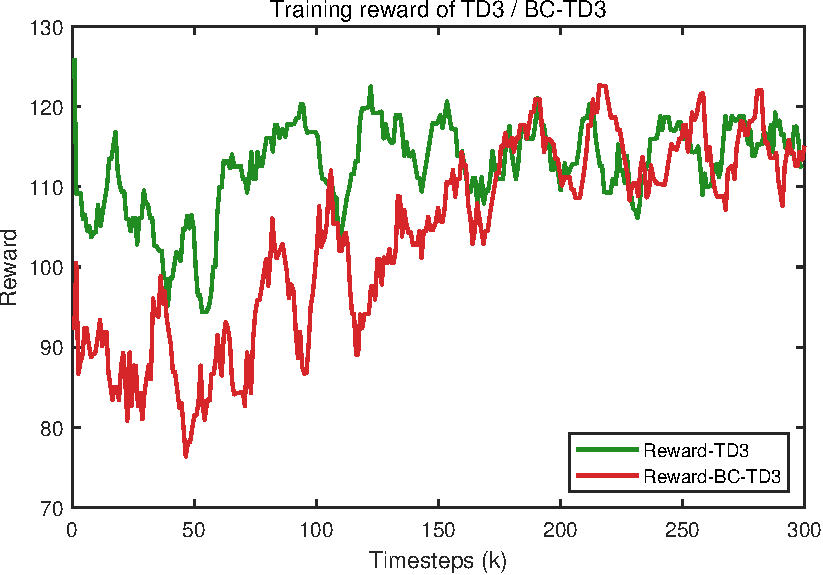
\includegraphics[width=0.68\linewidth]{fig03.pdf}
\caption{Training reward curves of BC-TD3 and TD3.}
\label{fig:reward}
\end{figure}

\Needspace{0.50\textheight}
The three-dimensional engagement trajectories of BC-TD3 and TD3 are shown in Fig.~\ref{fig:traj-bctd3} and Fig.~\ref{fig:traj-td3}.
\begin{figure}[H]
\centering
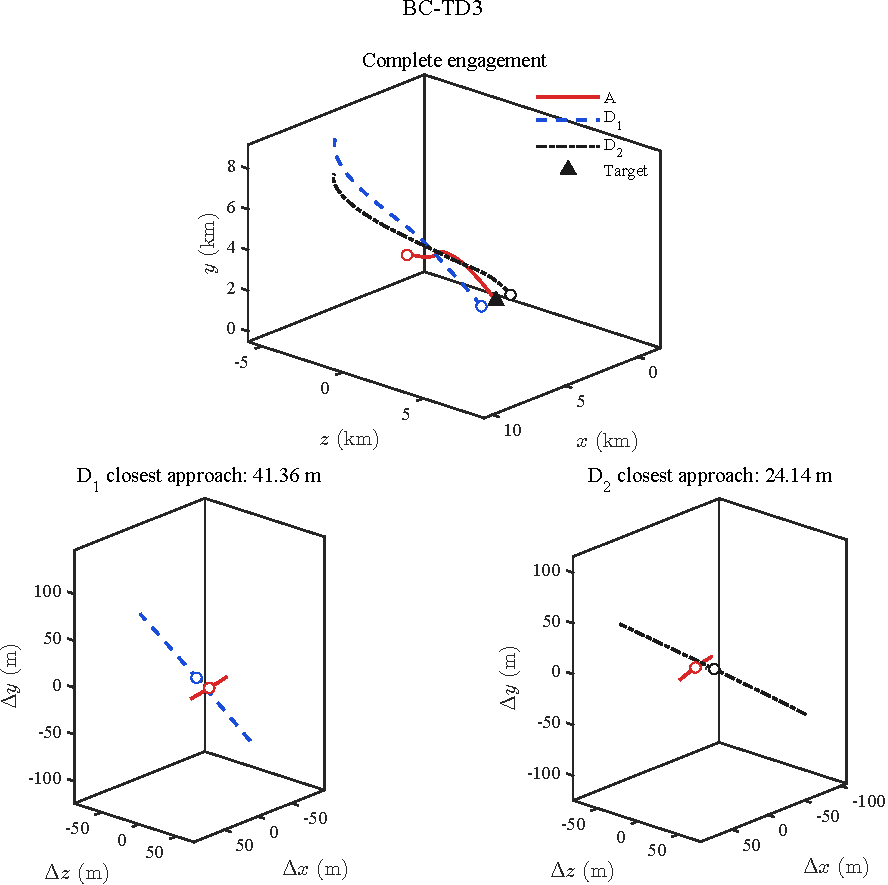
\includegraphics[width=0.64\linewidth]{fig04.pdf}
\caption{Three-dimensional BC-TD3 trajectory and enlarged views of the NCV encounters.}
\label{fig:traj-bctd3}
\end{figure}
\begin{figure}[H]
\centering
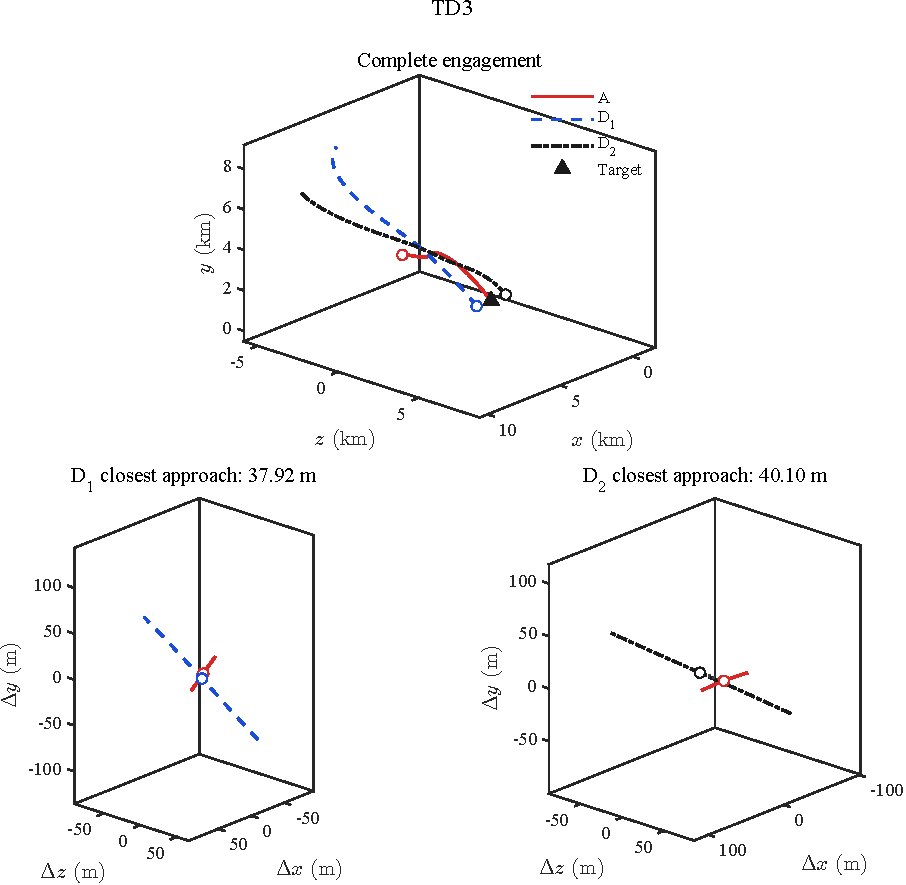
\includegraphics[width=0.64\linewidth]{fig05.pdf}
\caption{Three-dimensional TD3 trajectory and enlarged views of the NCV encounters.}
\label{fig:traj-td3}
\end{figure}

\Needspace{0.50\textheight}
The three-dimensional engagement trajectory of the sinusoidal maneuver is shown in Fig.~\ref{fig:traj-sine}.
\begin{figure}[H]
\centering
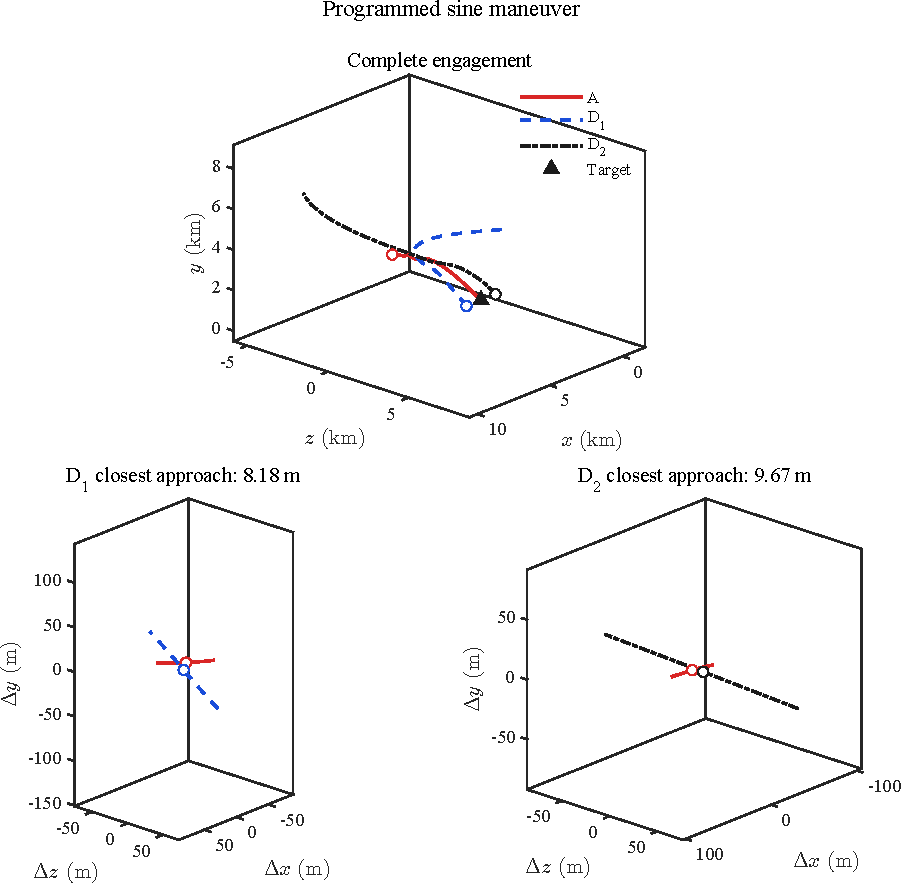
\includegraphics[width=0.64\linewidth]{fig06.pdf}
\caption{Three-dimensional trajectory of the sinusoidal maneuver and enlarged views of the NCV encounters.}
\label{fig:traj-sine}
\end{figure}

\Needspace{0.46\textheight}
The acceleration histories of the four guidance methods are shown in Fig.~\ref{fig:acc}.
\begin{figure}[H]
\centering
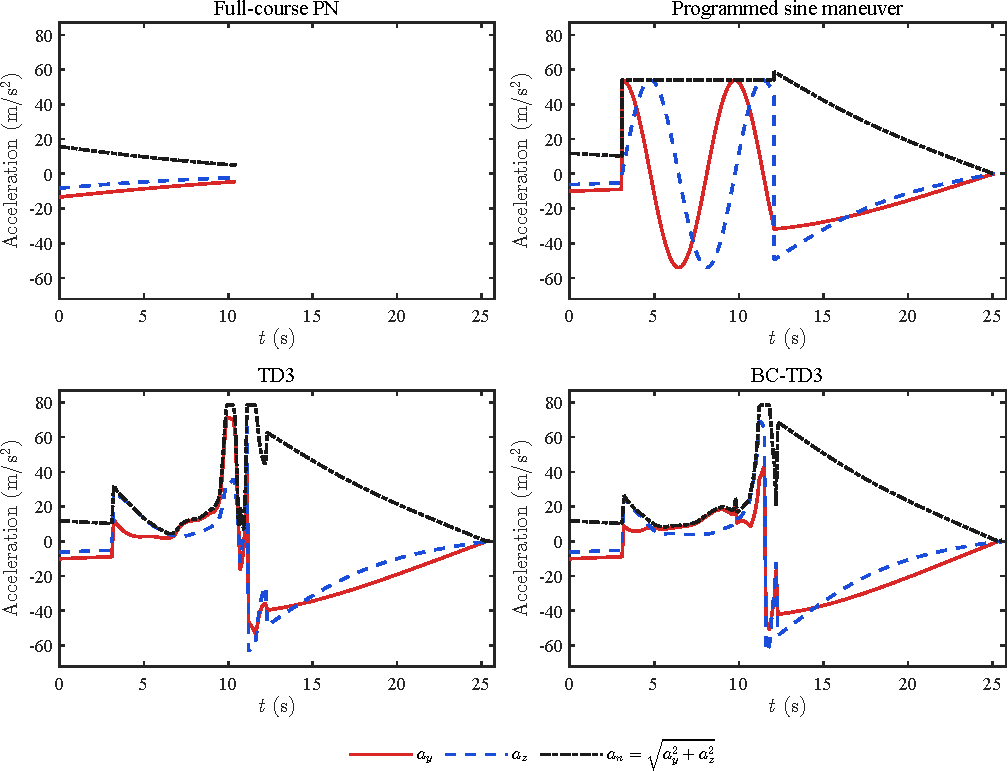
\includegraphics[width=0.78\linewidth]{fig07.pdf}
\caption{Normal acceleration histories of the compared methods.}
\label{fig:acc}
\end{figure}

\Needspace{0.46\textheight}
The histories of ${r_{AD1}}$, ${r_{AD2}}$, and ${r_{AT}}$ for the four guidance methods are shown in Fig.~\ref{fig:range}.
\begin{figure}[H]
\centering
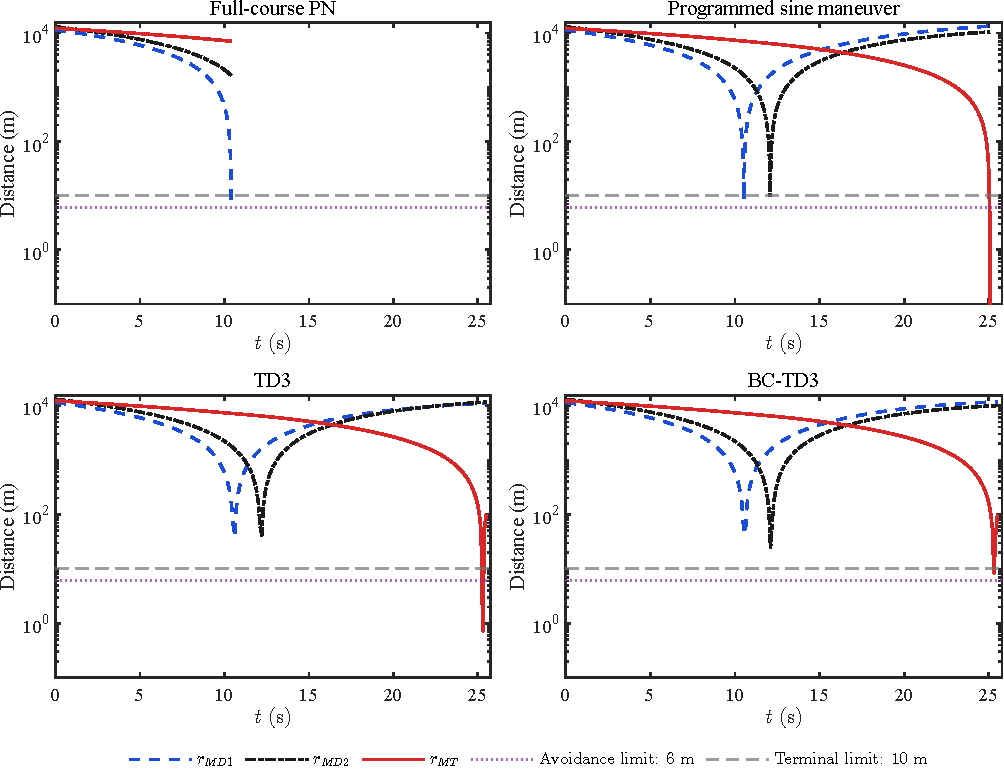
\includegraphics[width=0.78\linewidth]{fig08.pdf}
\caption{Range histories between the evader and the two NCVs and the target.}
\label{fig:range}
\end{figure}
From Fig.~\ref{fig:acc}--\ref{fig:range}, under full-course proportional navigation the evader flies nearly level with a small load factor. At about 10.5~s, ${r_{AD1}}$ reaches the evasion threshold (6~m), evasion fails, the simulation terminates early, and target-arrival guidance is not completed. The programmed sinusoidal maneuver applies a sustained large sinusoidal load factor in the middle phase, and ${a_n}$ remains high for a long time. The minimum values of ${r_{AD1}}$ and ${r_{AD2}}$ are both slightly above 6~m, and ${r_{AT}}$ falls below 10~m in the terminal phase, so evasion and target arrival can both be completed, but the safety margin relative to the NCVs is small. TD3 and BC-TD3 adaptively increase the maneuver in the middle phase. Near 10--12~s, ${a_n}$ reaches the $8g$ magnitude limit and then the load factor gradually decreases into terminal guidance. For both methods, the minimum values of ${r_{AD1}}$ and ${r_{AD2}}$ are clearly larger than those of the programmed maneuver, and the terminal ${r_{AT}}$ is below 10~m, so both complete dual-NCV evasion and target-arrival guidance. The maneuver of BC-TD3 is smoother and more stable.

To compare performance, 300 Monte Carlo simulations were run for BC+TD3, TD3, proportional navigation, and the programmed evasive maneuver. The comparison is given in Table~\ref{tab:perf-nonoise}.

\begin{table}[H]
\centering
\caption{Algorithm performance comparison (without noise).}
\label{tab:perf-nonoise}
\small
\begin{tabularx}{\linewidth}{lXX}
\toprule
Method & Dual-NCV evasion success rate $\min ({r_{AD1}},{r_{AD2}}) \geqslant 6{\text{m}}$ & Target-arrival success rate (evasion success and ${r_{AT,end}} \leqslant 10{\text{m}}$) \\
\midrule
Proportional navigation to the target only & 0.0\% & 0.0\% \\
Programmed maneuver (sinusoidal) & 76.3\% & 74.3\% \\
TD3 & 93.7\% & 93.0\% \\
BC+TD3 & 94.7\% & 94.3\% \\
\bottomrule
\end{tabularx}
\end{table}
Without a maneuver, or with only a fixed programmed maneuver, the evader has difficulty completing dual-NCV evasion and target arrival at the same time. Under proportional navigation to the target only, both success rates are 0.0\%. The programmed sinusoidal maneuver raises the two indices to 76.3\% and 74.3\%, which is still clearly insufficient. TD3 and BC+TD3 both complete the evasion and target-arrival guidance tasks well: the evasion and target-arrival success rates of TD3 are 93.7\% and 93.0\%, and BC+TD3 further reaches 94.7\% and 94.3\%. BC+TD3 is higher than TD3 on both success rates, and its overall performance and engineering applicability are better.

\subsection{Evasion and guidance under measurement noise}
% AGENT WARNING: the identification success rates in this subsection (especially 96.7\%/96.0\% with identification) are manually entered temporary placeholders, and the identification parameters in Section 6.1 are also temporary. Ignore these noisy-identification results and do not treat them as established evidence. Real results are of a similar magnitude. Do not conclude from them that the experiments as a whole have not succeeded, and do not weaken the contributions while writing. The Section 6.2 results without noise and identification are real results. See the AGENT WARNING at the start of this section.
In a practical engagement, the matrix elements required by the guidance law \eqref{eq:48} cannot be obtained from noise-free kinematics. As in \cref{asm:meas-noise}, onboard line-of-sight angles, line-of-sight rates, and attitude angles are corrupted by Gaussian white noise, while relative range and range rate are corrupted by Gaussian white noise of a relatively smaller magnitude. Substituting the angular measurements into \eqref{eq:13} and \eqref{eq:15} introduces biased and mutually correlated matrix errors. This subsection therefore repeats the engagement study under sensor noise and examines whether the sparse FF-RLS identifier of Section~4 can recover closed-loop performance. Two results are given: (i) a typical noisy BC-TD3 trajectory with online identification and enlarged encounter views; and (ii) a Monte Carlo comparison of five policies, namely BC-TD3 without and with identification, TD3, the sinusoidal maneuver, and PN.

\Needspace{0.52\textheight}
Fig.~\ref{fig:traj-id} shows a typical noisy flight trajectory of BC-TD3 combined with online sparse FF-RLS identification. The initial condition is based on Table~\ref{tab:init-traj}, and the noise intensity is the same as in Section~6.1, namely ${\sigma _q} = {\sigma _\theta } = {\sigma _\psi } = {3^ \circ }$, ${\sigma _{\dot q}} = 0.03{\text{rad/s}}$, ${\sigma _r} = 5{\kern 1pt} {\text{m}}$, and ${\sigma _{\dot r}} = 0.5{\kern 1pt} {\text{m/s}}$.
\begin{figure}[H]
\centering
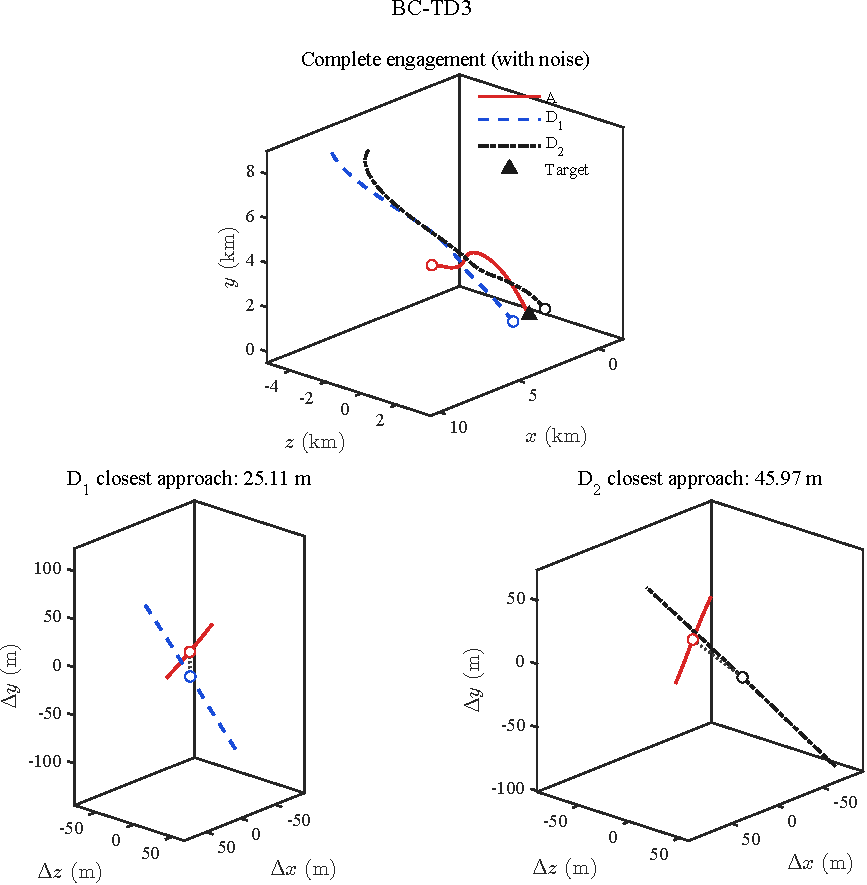
\includegraphics[width=0.64\linewidth]{fig09.pdf}
\caption{Three-dimensional trajectory of BC-TD3 with identification and enlarged encounter views (with measurement noise).}
\label{fig:traj-id}
\end{figure}

\Needspace{0.50\textheight}
A typical noisy flight trajectory without online sparse FF-RLS identification is shown in Fig.~\ref{fig:traj-noid}.
\begin{figure}[H]
\centering
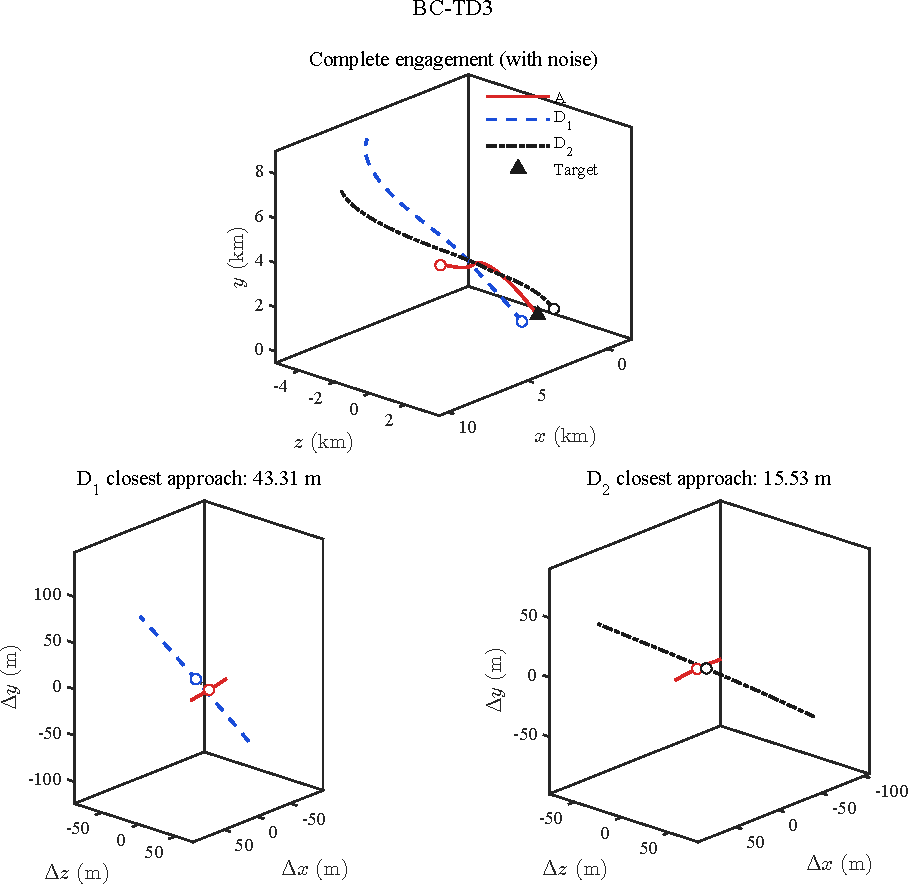
\includegraphics[width=0.64\linewidth]{fig10.pdf}
\caption{Three-dimensional trajectory of BC-TD3 without identification and enlarged encounter views (with measurement noise).}
\label{fig:traj-noid}
\end{figure}
From Fig.~\ref{fig:traj-id}--\ref{fig:traj-noid}, after the measurement noise above is introduced and processed by online sparse FF-RLS identification, the overall guidance and flight are almost unaffected: the evader can still complete a large maneuver, arrive at the target accurately, and maintain effective evasion. Without identification, the measurement noise enters the guidance loop directly. The closest evasion distances are 43.31~m and 15.53~m. The evasion distance from the second NCV ${D_2}$ decreases markedly, and the terminal target-arrival accuracy is also affected to some extent. Thus, without online sparse FF-RLS identification, both evasion and target-arrival performance degrade, whereas identification effectively suppresses the disturbance of measurement noise on evasion and target-arrival guidance.

The Monte Carlo results under measurement noise are given in Table~\ref{tab:perf-noise}.

\begin{table}[H]
\centering
\caption{Algorithm performance comparison (with noise).}
\label{tab:perf-noise}
\small
\begin{tabularx}{\linewidth}{lXX}
\toprule
Method (without identification unless noted) & Dual-NCV evasion success rate $\min ({r_{AD1}},{r_{AD2}}) \geqslant 6{\text{m}}$ & Target-arrival success rate (evasion success and ${r_{AT,end}} \leqslant 10{\text{m}}$) \\
\midrule
Proportional navigation to the target only & 0.0\% & 0.0\% \\
Programmed maneuver (sinusoidal) & 76.3\% & 74.3\% \\
TD3 & 92.3\% & 91.7\% \\
BC+TD3 & 93.7\% & 93.3\% \\
BC+TD3 with identification & 96.7\% & 96.0\% \\ % AGENT-PLACEHOLDER: temporary placeholder for the noisy-identification Monte Carlo. Real results are of a similar magnitude, but do not treat this row as established evidence, and do not infer that the experiments as a whole have not succeeded. See the warning at the start of this section.
\bottomrule
\end{tabularx}
\end{table}
Under measurement noise, the evader still has difficulty completing dual-NCV evasion and target arrival at the same time if it does not maneuver or uses only a fixed programmed maneuver. Under proportional navigation to the target only, both success rates are 0.0\%. The programmed sinusoidal maneuver raises the two indices to 76.3\% and 74.3\%, which is still clearly insufficient. The evasion and target-arrival success rates of TD3 and BC+TD3 are 92.3\% and 91.7\%, and 93.7\% and 93.3\%, respectively. They can still complete the task, but both are slightly lower than in the noise-free case. After online sparse FF-RLS parameter identification is introduced, BC+TD3 with identification further raises the two success rates to 96.7\% and 96.0\%, which is markedly higher than BC+TD3 without identification. This indicates that parameter identification can suppress measurement-noise disturbance and improve the robustness of evasion and target-arrival guidance.
% AGENT-PLACEHOLDER: the previous sentence, including 96.7\%/96.0\% and ``markedly higher'', is a temporary placeholder for the noisy-identification results and must not be treated as established evidence. Real results are of a similar magnitude. This note does not mean that the experiments as a whole have not succeeded, and it must not be used to weaken the writing position. The Section 6.2 results without noise and identification are real results. See the AGENT WARNING at the start of this section.
